\documentclass[aspectratio=169,10pt]{beamer}

\usetheme{Madrid}
\usecolortheme{seahorse}
\usefonttheme{professionalfonts}
\setbeamertemplate{footline}[frame number]
\setbeamertemplate{navigation symbols}{}

%--------------------------------------------------------------
% Packages
%--------------------------------------------------------------
\usepackage{amsmath,amssymb,amsfonts}
\usepackage{mathtools}
\usepackage{bm}
\usepackage{booktabs}
\usepackage{graphicx}
\usepackage{listings}
\usepackage{xcolor}
\usepackage{tikz}
\usepackage{array}
\usepackage{multicol}

\graphicspath{{figures/}}

%--------------------------------------------------------------
% Listings: Python style
%--------------------------------------------------------------
\lstdefinestyle{python}{
  language=Python,
  basicstyle=\ttfamily\scriptsize,
  numbers=left,
  numberstyle=\tiny\color{gray},
  frame=single,
  backgroundcolor=\color{gray!7},
  keywordstyle=\color{blue}\bfseries,
  commentstyle=\color{green!50!black}\itshape,
  stringstyle=\color{red!70!black},
  breaklines=true,
  tabsize=2,
  showstringspaces=false,
  captionpos=b,
}
\lstset{style=python}

%--------------------------------------------------------------
% Convenience macros
%--------------------------------------------------------------
\newcommand{\P}{\mathbb{P}}
\newcommand{\E}{\mathbb{E}}
\newcommand{\R}{\mathbb{R}}
\newcommand{\calP}{\mathcal{P}}
\newcommand{\calQ}{\mathcal{Q}}
\newcommand{\calN}{\mathcal{N}}

%--------------------------------------------------------------
% Title
%--------------------------------------------------------------
\title[E-Values -- Ch.5]{Hypothesis Testing with E-Values}
\subtitle{Chapter 5: The Universal Inference E-Value}
\author{Based on Ramdas \& Wang}
\date{}

\begin{document}

%--------------------------------------------------------------
\begin{frame}
  \titlepage
\end{frame}

%--------------------------------------------------------------
\begin{frame}{Table of Contents}
  \tableofcontents
\end{frame}

%==============================================================
\section{Notation and motivation (5.1)}
%==============================================================

\begin{frame}[allowframebreaks]{Notation you'll need}

  We assume familiarity with e-values/e-variables and p-values from
  earlier chapters. Here is everything new in this chapter, defined
  plainly.

  \begin{block}{Composite hypothesis}
    A hypothesis is \textbf{simple} if it names a single distribution
    (e.g.\ $H_0: p = N(0,1)$). It is \textbf{composite} if it names a
    whole \emph{set} of candidate distributions, $\calP$ for the null
    or $\calQ$ for the alternative (e.g.\ $H_0: p = N(\mu,1)$ for
    \emph{some unknown} $\mu \in \R$). Composite hypotheses are the
    realistic case: we almost never know the true parameter value in
    advance.
  \end{block}

  \begin{block}{Maximum likelihood estimator (MLE)}
    Given data $X_1,\ldots,X_m$ and a family of densities
    $\{p_\theta\}$, the MLE is the parameter value
    $\hat\theta = \arg\max_\theta \prod_{i=1}^m p_\theta(X_i)$ that
    makes the observed data as likely as possible. Equivalently it
    maximizes $\prod_i p(X_i)$ over $p$ ranging over a set $\calP$ of
    candidate densities (not necessarily indexed by a Euclidean
    parameter).
  \end{block}

  \framebreak

  \begin{block}{``Irregular model'' (plain meaning)}
    Classical hypothesis testing theory (Wilks' theorem, asymptotic
    normality of the MLE, chi-squared limits for likelihood ratios)
    relies on \emph{regularity conditions}: e.g.\ the number of
    parameters is fixed and small, the true parameter is an interior
    point, and the Fisher information matrix is invertible. A model is
    \textbf{irregular} when one or more of these fail -- for instance:
    \begin{itemize}
      \item a parameter is only identifiable under the alternative but
        not under the null (or vice versa),
      \item the true parameter sits on the boundary of the parameter
        space,
      \item the number of parameters grows with the sample size,
      \item the log-likelihood ratio statistic is not asymptotically
        $\chi^2$.
    \end{itemize}
    In irregular models, standard asymptotic tests may simply not have
    any known, provably valid version -- even approximately, even as
    $n\to\infty$.
  \end{block}

  \framebreak

  \begin{block}{Exchangeable data}
    A sequence $Z_1, Z_2, \ldots$ is \textbf{exchangeable} if the joint
    distribution of any finite subvector
    $(Z_1,\ldots,Z_n)$ is unchanged under any reordering (permutation)
    of the indices. iid data is exchangeable; so are repeated copies of
    the same random variable. Exchangeability is weaker than iid-ness
    but strong enough to support powerful concentration-free
    inequalities, as we'll see in Section 5.4.
  \end{block}

  \begin{alertblock}{The universal inference idea, in one sentence}
    If you can compute (or upper bound) the maximum likelihood under
    the null hypothesis, you can turn that single computation into a
    valid e-variable -- and hence a valid test -- for a composite null
    against a composite alternative, with \emph{no regularity
    conditions whatsoever}.
  \end{alertblock}

\end{frame}

%--------------------------------------------------------------
\begin{frame}[allowframebreaks]{5.1 Motivation: irregular models}

  \textbf{Why do we need a new tool at all?} For simple nulls we
  already know how to build e-variables (earlier chapters): just use a
  likelihood ratio against a fixed alternative. The trouble starts when
  \emph{both} the null and the alternative are composite -- then there
  is no unique ``the'' likelihood ratio, and classical theory (based on
  asymptotics of the MLE) may not even apply.

  \begin{exampleblock}{Motivating example 1: testing for a mixture}
    Let $p_{\mu_1,\mu_2,\lambda}$ be the density of
    $(1-\lambda)N(\mu_1,1) + \lambda N(\mu_2,1)$ (a two-component
    Gaussian mixture). Consider testing
    $$ H_0: \lambda = 0 \quad\text{(equivalently } \mu_1 = \mu_2 \text{)}
       \qquad\text{vs.}\qquad H_1: \text{unrestricted (except } \neq H_0). $$
    This is a genuinely composite null (any $\mu_1=\mu_2$ value is
    allowed) versus a genuinely composite alternative. It is also
    \emph{irregular}: under $H_0$ the parameter $\mu_2$ is not
    identified (any value of $\mu_2$ gives the same null distribution
    once $\lambda=0$), and under $H_1$, $\lambda$ is not identified as
    $\mu_1\to\mu_2$. This breaks the standard machinery (no
    $\chi^2$ limit for the likelihood ratio test), and to the authors'
    knowledge, universal inference gives the first test here with a
    provable type-I error guarantee.
  \end{exampleblock}

  \framebreak

  \begin{exampleblock}{Motivating example 2: shape constraints}
    A density $p$ on $\R$ is \textbf{log-concave} if $p = e^g$ for some
    concave function $g$ (log-concavity is a common, flexible
    nonparametric shape assumption -- it includes the Gaussian, the
    Laplace, the uniform, etc., but excludes heavy-tailed or strongly
    multimodal densities). Consider
    $$ H_0: p \text{ is log-concave} \qquad\text{vs.}\qquad H_1: p \text{ is not log-concave}. $$
    Both hypotheses are composite (they are sets of densities, not
    single densities), $\Theta$ is infinite-dimensional, and no other
    provably valid test for this problem is known. Universal inference
    applies directly, and is computationally efficient here because the
    log-concave MLE can be computed in polynomial time.
  \end{exampleblock}

  \begin{block}{The universal-inference reduction}
    Universal inference is a \emph{reduction}: it turns the (hard)
    problem of hypothesis testing under a composite null and
    alternative, with no regularity conditions, into the (often easier)
    problem of computing -- or just upper bounding -- the
    \textbf{maximum likelihood under the null}.
  \end{block}

  \textbf{Two standing assumptions for this chapter:}
  \begin{enumerate}
    \item $\calP$ (null) and $\calQ$ (alternative) share a common
      density scale, so every distribution can be represented by an
      ordinary density $p(x)$ or $q(x)$.
    \item The data is $X^n = (X_1,\ldots,X_n)$ with iid entries; we
      identify a distribution $\P \in \calP$ with the density $p(x)$ of
      a single coordinate, and use $p \in \calP$ and $\P \in \calP$
      interchangeably.
  \end{enumerate}

\end{frame}

%==============================================================
\section{Split likelihood ratio e-variable (5.2)}
%==============================================================

\begin{frame}{5.2 Intuition: why not just use the likelihood ratio directly?}

  \textbf{The obstacle.} For a simple null $p$ vs.\ a simple
  alternative $q$, the likelihood ratio $q(X)/p(X)$ is already a valid
  e-variable: $\E^p[q(X)/p(X)] = \int q(x)\,dx = 1$. So why not just
  plug in the MLE $\hat p$ under the (composite) null and the MLE
  $\hat q$ under the alternative, and use $\hat q(X^n)/\hat p(X^n)$?

  \begin{alertblock}{The problem}
    Under a composite null, we don't know the true $p \in \calP$. If we
    estimate $\hat p$ \emph{using the very same data} we test on, the
    ratio $\hat q(X^n)/\hat p(X^n)$ is no longer guaranteed to have
    expectation $\le 1$ -- $\hat p$ was chosen (in part) to explain that
    data, so it artificially inflates the likelihood ratio in its own
    favor. This double-use of the data breaks the e-variable property.
  \end{alertblock}

  \begin{block}{The fix: split the data}
    Split the sample into two independent halves. Use one half only to
    \emph{choose} a plausible alternative distribution. Use the other
    half only to \emph{fit the null MLE and evaluate the ratio}. Because
    the null MLE is honestly maximizing likelihood over the data it is
    tested against -- and only over that data -- the key inequality
    $\prod \hat p_0(X_i) \ge \prod p(X_i)$ becomes available, and it is
    exactly what restores the $\le 1$ expectation guarantee. This is the
    single trick behind the whole chapter.
  \end{block}

\end{frame}

%--------------------------------------------------------------
\begin{frame}{Step-by-step: building the split likelihood ratio e-variable}

  \begin{block}{Step 1 -- Split the data}
    Divide $X^n=(X_1,\ldots,X_n)$ into two \emph{independent} sets
    $D_0$ and $D_1$. E.g.\ let $I \subset [n]$ be a random subset
    independent of $X^n$ (flip an independent coin for each point), and
    set $D_0 = \{X_i : i \in I\}$, $D_1 = \{X_i : i \notin I\}$. Roughly
    equal sizes are a reasonable default, but validity does \emph{not}
    depend on the split proportion (only e-power does). The split need
    not even be random: $D_0=\{X_1,\ldots,X_m\}$, $D_1 = \{X_{m+1},\ldots,X_n\}$
    works too.
  \end{block}

  \begin{block}{Step 2 -- Pick a candidate alternative using $D_1$}
    Choose any $\hat q_1 \in \calQ$ based only on $D_1$: an MLE, a
    Bayes estimator (posterior mean/mode under some prior), or a robust
    estimator. This choice is \emph{unrestricted} -- it cannot affect
    validity, only power/e-power.
  \end{block}

  \begin{block}{Step 3 -- Fit the null MLE using $D_0$}
    $$ \hat p_0 = \arg\max_{p \in \calP} \prod_{i \in D_0} p(X_i). $$
    Here $\hat p_0$ is the density in the null family $\calP$ that best
    explains $D_0$ alone.
  \end{block}

\end{frame}

%--------------------------------------------------------------
\begin{frame}{The split likelihood ratio e-variable}

  \begin{block}{Step 4 -- Form the ratio, evaluated on $D_0$}
    $$ E \;=\; \prod_{i \in D_0} \frac{\hat q_1(X_i)}{\hat p_0(X_i)}. \qquad (5.1)$$
    \textbf{Symbols:} $D_0, D_1$ are the two (independent) halves of
    the data; $\hat q_1$ is the alternative fitted \emph{only} using
    $D_1$; $\hat p_0$ is the null MLE fitted \emph{only} using $D_0$;
    the product (equivalently, the ratio of the two ``likelihoods'') is
    evaluated over the points in $D_0$.
  \end{block}

  We call $E$ the \textbf{split likelihood ratio e-variable}. Note the
  asymmetric roles: $D_1$ only supplies the fixed candidate $\hat q_1$;
  $D_0$ is used twice -- once to fit $\hat p_0$, and once again (the
  same data!) to evaluate the ratio.

  \begin{alertblock}{Variant: cross-fit likelihood ratio e-variable}
    Swap the roles of $D_0,D_1$, recompute $E^{\text{swap}}$ by the same
    recipe, and average:
    $$ E^{\text{cross-fit}} = \frac{E + E^{\text{swap}}}{2}. $$
    Combined with Markov's inequality (Chapter 2) this yields the
    \emph{split LRT} or \emph{cross-fit LRT}: a level-$\alpha$ test that
    rejects $H_0$ when the e-variable exceeds $1/\alpha$.
  \end{alertblock}

\end{frame}

%--------------------------------------------------------------
\begin{frame}{Theorem 5.1: validity of the split LR e-variable}

  \begin{alertblock}{Theorem 5.1}
    The split likelihood ratio statistic $E$ defined in (5.1) is an
    e-variable for $\calP$: $\E^\P[E] \le 1$ for every $\P \in \calP$.
  \end{alertblock}

  \textbf{Why this deserves its own theorem:} it is what lets us plug
  $E$ into Markov's inequality and get a valid level-$\alpha$ test, no
  matter how irregular the model is, and no matter what estimator was
  used for $\hat q_1$.

  \begin{block}{Proof, step by step}
    \begin{enumerate}
      \item By definition, $\hat p_0$ maximizes $\prod_{i\in D_0} p(X_i)$
        over $p\in\calP$, so for \emph{any} $\P \in \calP$,
        $$ \prod_{i \in D_0} \hat p_0(X_i) \;\ge\; \prod_{i \in D_0} p(X_i). $$
      \item Dividing through (the numerator $\hat q_1(X_i)$ is common)
        and taking $\E^\P[\cdot \mid D_1]$:
        $$ \E^\P\!\left[\prod_{i\in D_0}\frac{\hat q_1(X_i)}{\hat p_0(X_i)} \,\middle|\, D_1\right]
           \;\le\; \E^\P\!\left[\prod_{i\in D_0}\frac{\hat q_1(X_i)}{p(X_i)} \,\middle|\, D_1\right] = 1. $$
      \item The final equality holds because, conditional on $D_1$,
        $\hat q_1$ is a \emph{fixed} density, $D_0 \perp D_1$, and a
        likelihood ratio of any fixed alternative to the true density
        $p$ is an exact e-variable with mean exactly $1$.
      \item Take a further expectation over $D_1$ and use the tower
        property: $\E^\P[E] = \E^\P\big[\E^\P[E\mid D_1]\big] \le 1$.
        $\blacksquare$
    \end{enumerate}
  \end{block}

\end{frame}

%--------------------------------------------------------------
\begin{frame}{Remark: mixture universal inference}

  \begin{block}{Remark 5.2 (mixture variant)}
    Instead of plugging in a single point estimate $\hat q_1$, use
    $D_1$ to choose a whole distribution $\nu$ over $\calQ$ (e.g.\ a
    Bayesian posterior), and define
    $$ E = \int_\calQ \prod_{i\in D_0} \frac{q(X_i)}{\hat p_0(X_i)}\, \nu(dq). $$
  \end{block}

  \textbf{Intuition:} the null side still uses the plug-in MLE
  $\hat p_0$, but the alternative side is now an \emph{average}
  (mixture) over candidate alternatives rather than a single plug-in
  estimate. Since an average of e-variables is again an e-variable
  (each $\prod_{i\in D_0} q(X_i)/\hat p_0(X_i)$ is itself a valid
  e-variable conditional on $D_1$, by the same argument as Theorem
  5.1), the mixture version is valid by an almost identical proof --
  integrals are just (possibly uncountable) averages. In practice, a
  prior with mass spread over all of $\calQ$ tends to help e-power,
  especially in small samples, and can be viewed simply as a smoothed
  version of the plug-in MLE.

\end{frame}

%--------------------------------------------------------------
\begin{frame}{Running example: Gaussian vs.\ Gaussian mixture}

  \textbf{Setup.} $H_0$: data are $N(\mu,1)$ (simple family, one
  unknown mean). $H_1$: data are a 2-component mixture
  $(1-\lambda)N(\mu_1,1)+\lambda N(\mu_2,1)$ with $\mu_1,\mu_2,\lambda$
  all free (this is exactly the irregular model of Section 5.1). We
  simulate $n=40$ points from a genuine mixture and split them
  $20/20$ into $D_0, D_1$.

  \begin{columns}
    \begin{column}{0.55\textwidth}
      \begin{block}{What we computed (one concrete run)}
        \begin{itemize}
          \item Null MLE on $D_0$ (sample mean, variance known $=1$):
            $\hat\mu_0 = 0.289$.
          \item Alternative fit on $D_1$ (2-component mixture MLE via
            numerical optimization):
            $\hat\mu_1 = 1.194,\ \hat\mu_2 = -0.667,\ \hat\lambda = 0.403$.
          \item Split LR e-variable, evaluated on $D_0$:
            $$ \log E = \sum_{i\in D_0}\Big[\log \hat q_1(X_i) - \log \hat p_0(X_i)\Big] = 5.655, $$
            i.e.\ $E \approx 285.8$.
        \end{itemize}
      \end{block}
      At $\alpha = 0.05$, since $E = 285.8 \gg 1/\alpha = 20$, the split
      LRT would reject $H_0$ here -- correctly, since the data really
      did come from a mixture.
    \end{column}
    \begin{column}{0.45\textwidth}
      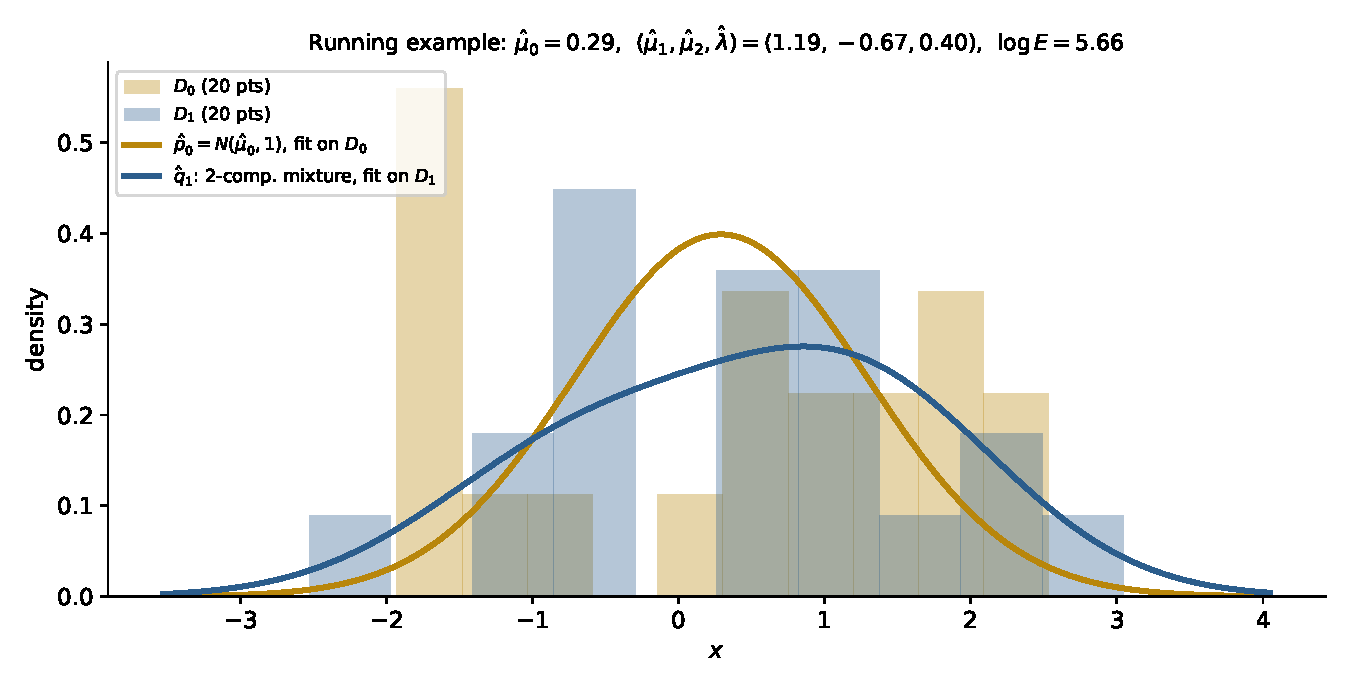
\includegraphics[width=\linewidth]{fig_running_example.pdf}
    \end{column}
  \end{columns}

\end{frame}

%--------------------------------------------------------------
\begin{frame}[fragile]{Python: split LR e-variable (5.2)}

  This reproduces the numbers on the previous slide: null MLE
  (sample mean) on $D_0$, a 2-component Gaussian mixture MLE on $D_1$
  (via numerical optimization), and the split LR e-variable.

\begin{lstlisting}[language=Python]
import numpy as np
from scipy.stats import norm
from scipy.optimize import minimize

def mixture_negloglik(params, x):
    mu1, mu2, lam = params
    lam = min(max(lam, 1e-6), 1 - 1e-6)
    dens = (1-lam)*norm.pdf(x, mu1, 1) + lam*norm.pdf(x, mu2, 1)
    return -np.sum(np.log(np.clip(dens, 1e-300, None)))

def split_LR_evariable(D0, D1):
    # Step 2: alternative fit on D1 (mixture MLE)
    res = minimize(mixture_negloglik, x0=[-1, 1, 0.5], args=(D1,),
                    method="Nelder-Mead")
    mu1_hat, mu2_hat, lam_hat = res.x
    # Step 3: null MLE on D0 (single Gaussian mean, var=1)
    mu0_hat = D0.mean()
    # Step 4: ratio, evaluated on D0
    q1 = (1-lam_hat)*norm.pdf(D0, mu1_hat, 1) + lam_hat*norm.pdf(D0, mu2_hat, 1)
    p0 = norm.pdf(D0, mu0_hat, 1)
    logE = np.sum(np.log(q1) - np.log(p0))
    return logE, np.exp(logE)

rng = np.random.default_rng(2024)
comp = rng.random(40) < 0.5
x = np.where(comp, rng.normal(1.2, 1, 40), rng.normal(-1.2, 1, 40))
idx = rng.permutation(40)
D0, D1 = x[idx[:20]], x[idx[20:]]
logE, E = split_LR_evariable(D0, D1)
print(f"log E = {logE:.3f}, E = {E:.3e}")   # matches the slide above
\end{lstlisting}

\end{frame}

%==============================================================
\section{Subsampled likelihood ratio e-variable (5.3)}
%==============================================================

\begin{frame}{5.3 Intuition: taming the randomness of splitting}

  \textbf{The obstacle.} The split LR e-variable introduces an extra
  source of randomness that has nothing to do with the data: the
  \emph{coin flips} used to decide the split. Two analysts with the
  exact same data $X^n$ but different random splits can get quite
  different values of $E$, and hence reach different conclusions. This
  ``algorithmic randomness'' is unsatisfying and can hurt e-power.

  \begin{block}{The fix: split many times and average}
    Recompute the split LR e-variable independently $B$ times, using
    $B$ fresh, iid random splits of the same data (these can all be
    computed in parallel), giving e-variables $E^{(1)},\ldots,E^{(B)}$.
    Average them:
    $$ \bar E^{(B)} = \frac{E^{(1)} + \cdots + E^{(B)}}{B}. \qquad (5.2)$$
    We call $\bar E^{(B)}$ the \textbf{subsampled likelihood ratio
    e-variable}. This is a form of \emph{Rao--Blackwellization}: we
    remove variance introduced by an artificial randomization device,
    by averaging over that device.
  \end{block}

  As a special case, $B=2$ with the two splits swapped recovers the
  \emph{cross-fit} likelihood ratio e-variable from Section 5.2.

\end{frame}

%--------------------------------------------------------------
\begin{frame}{Proposition 5.3: averaging can only help}

  \begin{alertblock}{Proposition 5.3 (improving e-power by averaging)}
    Let $E^{(1)},\ldots,E^{(B)}$ be \emph{arbitrary} e-variables (not
    necessarily split LR ones), and $\bar E^{(B)}$ their average. For
    any distribution $\mathbb{Q}$,
    $$ \E^{\mathbb{Q}}\big[\log \bar E^{(B)}\big] \;\ge\; \frac{1}{B}\sum_{b=1}^{B} \E^{\mathbb{Q}}\big[\log E^{(b)}\big], $$
    provided the right side is well defined. In particular, if
    $E^{(1)},\ldots,E^{(B)}$ are iid copies of the split LR e-variable
    (5.1), the subsampled e-variable (5.2) has e-power (against any
    $\mathbb{Q}$) at least as large as that of a single split LR
    e-variable.
  \end{alertblock}

  \textbf{Proof idea:} $\log(\cdot)$ is a concave function, so by
  Jensen's inequality $\log\!\big(\tfrac1B\sum_b E^{(b)}\big) \ge
  \tfrac1B\sum_b \log E^{(b)}$ pointwise; take $\E^{\mathbb Q}$ of both
  sides. That's it -- the whole argument is one line of concavity.
  As $B \to \infty$, $\bar E^{(B)}$ converges almost surely to a fixed
  limiting random variable (this uses the backward-martingale fact of
  Section 5.4).

\end{frame}

%--------------------------------------------------------------
\begin{frame}{The subsampled LRT: a sequential procedure}

  \begin{block}{Subsampled LRT}
    For $b \ge 1$, let $\bar E^{(b)} = (E^{(1)}+\cdots+E^{(b)})/b$. The
    subsampled LRT \textbf{rejects} $H_0$ as soon as any running
    average $\bar E^{(b)}$ exceeds $1/\alpha$, for any $b \ge 1$. One
    can compute $E^{(1)}, E^{(2)}, \ldots$ one split at a time, updating
    the running average $\bar E^{(1)}, \bar E^{(2)}, \ldots$
    sequentially, and stop (rejecting) at the first time any of these
    exceeds $1/\alpha$. Crucially, $B$ can be \emph{data-dependent}
    (e.g.\ ``keep splitting until convinced, or until compute budget
    runs out'') \emph{without} violating the type-I error guarantee.
  \end{block}

  \begin{alertblock}{Proposition 5.4}
    The subsampled LRT controls type-I error at level $\alpha$, and is
    at least as powerful as the (single-split) split LRT.
  \end{alertblock}

  The power claim is immediate: the very first step of the subsampled
  procedure, $b=1$, is exactly the split LRT. The type-I error claim is
  \emph{not} obvious -- naively, ``keep testing until you reject'' looks
  like it should inflate type-I error (optional stopping). It doesn't
  here, and the reason is the \textbf{exchangeable Markov inequality} of
  Section 5.4, coming up next.

\end{frame}

%--------------------------------------------------------------
\begin{frame}[fragile]{Python: subsampled / cross-fit LR e-variable (5.3)}

  A running average of independently split LR e-variables, stopped the
  first time it crosses $1/\alpha$ (sequential subsampled LRT).

\begin{lstlisting}[language=Python]
import numpy as np

def subsampled_LRT(x, alpha, B_max, split_lr_fn, rng):
    """x: full data array. split_lr_fn(D0, D1, rng) -> log E for one split.
    Returns (rejected: bool, b_stop: int or None, running_Ebar: list)."""
    n = len(x)
    logEs, Ebars = [], []
    for b in range(1, B_max + 1):
        idx = rng.permutation(n)
        half = n // 2
        D0, D1 = x[idx[:half]], x[idx[half:]]
        logEs.append(split_lr_fn(D0, D1, rng))
        Ebar = np.mean(np.exp(logEs))          # average of E's, not of logE's
        Ebars.append(Ebar)
        if Ebar >= 1 / alpha:                  # exchangeable Markov guarantee
            return True, b, Ebars              # kicks in here -- see Sec. 5.4
    return False, None, Ebars

# Example: split_lr_fn could wrap the split_LR_evariable() from the
# previous slide and return only its logE.
rng = np.random.default_rng(1)
split_lr_fn = lambda D0, D1, rng: split_LR_evariable(D0, D1)[0]
rejected, b_stop, Ebars = subsampled_LRT(x, alpha=0.05, B_max=20,
                                         split_lr_fn=split_lr_fn, rng=rng)
print("rejected:", rejected, " at split #", b_stop)
\end{lstlisting}

\end{frame}

%==============================================================
\section{Exchangeable Markov's inequality (5.4)}
%==============================================================

\begin{frame}{5.4 Intuition: why do we need a new inequality?}

  \textbf{The obstacle.} Ordinary Markov's inequality,
  $\P(Z \ge 1/\alpha) \le \alpha\,\E[Z]$ for $Z\ge 0$, is a
  \emph{one-shot} guarantee: it bounds the chance of a single random
  variable being large. But the subsampled LRT looks at a whole
  \emph{running average} $\bar E^{(1)}, \bar E^{(2)}, \ldots$ and
  rejects if \emph{any} of them ever crosses the threshold -- this is
  an ``optional stopping''-flavored claim, and plain Markov does not
  cover it.

  \begin{block}{The fix: exploit exchangeability}
    $E^{(1)}, E^{(2)}, \ldots$ (the repeated, independent-split
    e-variables) are not just any random variables: they are
    \textbf{exchangeable} -- reordering the splits doesn't change their
    joint distribution, since the splits are iid. It turns out
    exchangeability alone (no independence needed) is exactly enough
    structure to control the \emph{whole trajectory} of running
    averages, via a \emph{backward martingale} argument.
  \end{block}

  \begin{block}{Definition: exchangeable sequence}
    $Z_1,\ldots,Z_n$ are exchangeable if $(Z_1,\ldots,Z_n) \stackrel{d}{=} (Z_{\pi(1)},\ldots,Z_{\pi(n)})$
    for every permutation $\pi$ of $\{1,\ldots,n\}$. An infinite
    sequence is exchangeable if every finite subsequence is.
  \end{block}

\end{frame}

%--------------------------------------------------------------
\begin{frame}{Fact 5.5 and Theorem 5.6 (EMI)}

  \begin{block}{Fact 5.5 (backward martingale)}
    For any exchangeable, integrable sequence $Z_1,Z_2,\ldots$, the
    running-mean process $\bar Z_n := (Z_1+\cdots+Z_n)/n$ is a
    \textbf{backward martingale}: with $\mathcal{G}_{n+1} :=
    \sigma(\bar Z_{n+1}, \bar Z_{n+2}, \ldots)$ (information from index
    $n+1$ onward),
    $$ \E^\P[\bar Z_n \mid \mathcal{G}_{n+1}] = \bar Z_{n+1} \quad \text{for all } n. $$
    Moreover $\bar Z_n$ converges almost surely to an integrable random
    variable as $n \to \infty$ (this is Doob's backward martingale
    convergence theorem).
  \end{block}

  \begin{alertblock}{Theorem 5.6: Exchangeable Markov Inequality (EMI)}
    For any exchangeable sequence $Z_1, Z_2, \ldots$ and any $\alpha > 0$,
    $$ \P\left(\sup_{n\ge 1} \left|\frac{1}{n}\sum_{i=1}^n Z_i\right| \ge \frac{1}{\alpha}\right) \le \alpha\, \E^\P[|Z_1|]. \qquad (5.3)$$
    In particular, if $Z_1, Z_2, \ldots$ are e-variables,
    $$ \P\left(\exists n \ge 1 : \frac{1}{n}\sum_{i=1}^n Z_i \ge \frac1\alpha \right) \le \alpha. $$
  \end{alertblock}

  \textbf{Symbols:} $\sup_{n\ge1}$ -- the \emph{worst case over all
  sample sizes ever looked at}, not just one fixed $n$; this is exactly
  the ``look at the whole trajectory'' guarantee the subsampled LRT
  needs. The proof combines Fact 5.5 with a time-reversed Ville's
  inequality (Chapter 7).

\end{frame}

%--------------------------------------------------------------
\begin{frame}{Turning arbitrary dependence into exchangeability}

  \textbf{Why this matters:} EMI needs exchangeability, but many
  real datasets are only iid, or not even that. A simple trick --
  random permutation -- manufactures exchangeability out of thin air.

  \begin{block}{Corollary: random-permutation trick}
    Let $Z_1,\ldots,Z_n$ be \emph{arbitrarily dependent} (not
    necessarily exchangeable), let $\pi$ be an independent uniformly
    random permutation of $\{1,\ldots,n\}$. Then for any $\alpha>0$,
    $$ \P\left(\sup_{1\le m\le n} \frac1m \sum_{i=1}^m |Z_{\pi(i)}| \ge \frac1\alpha\right)
       \le \alpha\, \frac{\E^\P[|Z_1|+\cdots+|Z_n|]}{n}. $$
    Randomly permuting the (otherwise arbitrary) sequence makes it
    exchangeable \emph{by construction}, so (5.3) applies to
    $Z_{\pi(1)},\ldots,Z_{\pi(n)}$.
  \end{block}

  \begin{block}{Variant: sampling from a bag}
    Take $N$ arbitrarily dependent random variables, put them in a
    bag, and draw $n \le N$ of them uniformly at random (with or
    without replacement) as $Z_{\pi(1)}, \ldots, Z_{\pi(n)}$. Then
    $$ \P\left(\sup_{1\le m\le n} \frac1m \sum_{i=1}^m |Z_{\pi(i)}| \ge \frac1\alpha\right)
       \le \alpha\, \frac{\E^\P[|Z_1|+\cdots+|Z_N|]}{N}. $$
    The random sampling process itself induces the exchangeability
    needed to invoke (5.3), even though the original bag of $N$
    variables need not be exchangeable.
  \end{block}

\end{frame}

%--------------------------------------------------------------
\begin{frame}{Theorem 5.7: Exchangeable Uniformly Randomized MI (EUMI)}

  \begin{alertblock}{Theorem 5.7 (EUMI)}
    Let $Z_1,\ldots,Z_n$ be exchangeable. Then for any $a \in (0,1)$,
    $$ \P\left(Z_1 \ge U/a \ \text{ or }\ \exists\, t\le n:\ \left|\sum_{i=1}^t Z_i / t\right| \ge 1/a\right)
       \le a \cdot \E^\P[|Z_1|], $$
    where $U$ is a uniform random variable on $[0,1]$, independent of
    $Z_1,\ldots,Z_n$.
  \end{alertblock}

  \textbf{Why bother with the extra $U$?} This combines the running-average
  guarantee (Theorem 5.6) with the \emph{uniformly randomized} Markov
  inequality (a sharper, randomized version of Markov's inequality
  introduced in Chapter 2, which can strictly increase power at the
  cost of injecting independent external randomness $U$). In the
  numerical studies of Section 5.7, using this randomized threshold in
  place of the plain Markov threshold noticeably improves power (the
  ``UMI''/``EUMI'' variants), at the modest cost of extra
  randomization.

\end{frame}

%--------------------------------------------------------------
\begin{frame}[fragile]{Python: exchangeable Markov's inequality, demonstrated}

  A quick simulation confirming that the trajectory-wide guarantee
  (5.3) actually holds for an exchangeable sequence of e-variables
  (here, iid log-normal e-variables with mean $1$).

\begin{lstlisting}[language=Python]
import numpy as np

rng = np.random.default_rng(0)
alpha, n_steps, reps = 0.05, 500, 20000
sigma = 1.0
exceed_count = 0
for _ in range(reps):
    # iid e-variable: E[Z]=1 by construction (lognormal, mean-corrected)
    Z = np.exp(rng.normal(-sigma**2/2, sigma, n_steps))
    running_mean = np.cumsum(Z) / np.arange(1, n_steps + 1)
    if np.any(running_mean >= 1/alpha):
        exceed_count += 1
print(f"P(sup_n running_mean >= 1/alpha) ~= {exceed_count/reps:.4f}")
print(f"EMI bound: alpha = {alpha}")   # empirical rate should be <= alpha
\end{lstlisting}

  Running this shows the empirical exceedance rate safely below
  $\alpha=0.05$ -- Theorem 5.6 is not just valid but often quite loose
  in this iid case, which is expected since (5.3) has to hold for
  \emph{every} exchangeable sequence, including adversarial ones.

\end{frame}

%==============================================================
\section{Universal confidence sets (5.5)}
%==============================================================

\begin{frame}{5.5 Intuition: from tests to confidence sets, for free}

  \textbf{Setup.} Suppose distributions are indexed by a parameter,
  $\{p_\theta\}_{\theta\in\Theta}$, and the true parameter is
  $\theta^*$. A $(1-\alpha)$ confidence set is a data-dependent set
  $C(X^n)$ such that $\P_{\theta^*}(\theta^* \in C(X^n)) \ge 1-\alpha$
  for every possible $\theta^* \in \Theta$.

  \begin{block}{The standard trick: test inversion}
    Test \emph{every single point} $\theta \in \Theta$ as if it were a
    simple null (``$H_0: \theta^*=\theta$'') at level $\alpha$, and
    collect all the $\theta$'s that survive (are not rejected). Because
    each individual test has type-I error $\le \alpha$, the true
    $\theta^*$ survives its own point-null test with probability
    $\ge 1-\alpha$ -- so the collected set covers $\theta^*$ with
    probability $\ge 1-\alpha$. This works for \emph{any} valid test,
    with no regularity conditions -- so it works for the split LRT.
  \end{block}

  \textbf{Why this is attractive here:} classical confidence sets
  usually need asymptotic normality of an estimator, or a known
  sampling distribution for a test statistic. Universal inference
  needs neither.

\end{frame}

%--------------------------------------------------------------
\begin{frame}{Constructing the universal confidence set}

  Split $X^n$ into $D_0, D_1$ as before. Let $\hat\theta$ be any
  estimator computed from $D_1$ alone. Define
  $$ C(X^n) := \left\{\theta \in \Theta \,:\, \prod_{i\in D_0} \frac{p_{\hat\theta}(X_i)}{p_\theta(X_i)} < \frac1\alpha \right\}. $$

  \begin{block}{Notation}
    Write $\mathcal{L}_0(\theta) := \prod_{i \in D_0} p_\theta(X_i)$ for
    the (null-family) likelihood evaluated on $D_0$ alone. Then
    $$ C(X^n) = \left\{\theta \in \Theta \,:\, \mathcal{L}_0(\hat\theta)/\mathcal{L}_0(\theta) < 1/\alpha\right\}. $$
    In words: $\theta$ is in the confidence set exactly when the point
    hypothesis $\theta^*=\theta$ is \emph{not rejected} by the split LRT
    that compares $\hat\theta$ (fit on $D_1$) against $\theta$ (using
    $D_0$).
  \end{block}

  \begin{alertblock}{Proposition 5.8}
    For any $\theta^* \in \Theta$ and any predefined $\alpha \in (0,1)$,
    $C(X^n)$ above is a $(1-\alpha)$ confidence set for $\theta^*$.
  \end{alertblock}

  The proof is immediate from Theorem 5.1: for the true $\theta^*$,
  $E = \mathcal{L}_0(\hat\theta)/\mathcal{L}_0(\theta^*)$ is an
  e-variable, so $\mathbb 1_{\{E \ge 1/\alpha\}}$ is a level-$\alpha$
  test, and $\theta^*$ fails to be excluded from $C(X^n)$ with
  probability $\ge 1-\alpha$.

\end{frame}

%--------------------------------------------------------------
\begin{frame}{Example: multivariate Gaussian mean, identity covariance}

  Let $X_1,\ldots,X_n \stackrel{\text{iid}}{\sim} N(\theta^*, I_d)$.
  Here $C(X^n)$ turns out to be a Euclidean ball (spherical confidence
  region) around $\hat\theta$. A natural question: what fraction
  $p_0$ of the data should go into $D_0$ (used for the ratio) versus
  $D_1$ (used to compute $\hat\theta$)?

  \begin{alertblock}{Theorem 5.9: optimal splitting proportion}
    The splitting proportion $p_0^*$ that minimizes the expected squared
    radius $\E^\P[r^2(C(X^n))]$ of the confidence set is
    $$ p_0^* = 1 - \frac{\sqrt{4d^2 + 8d\log(1/\alpha)} - 2d}{4\log(1/\alpha)}. $$
  \end{alertblock}

  \textbf{Reading the formula:} $d$ is the dimension, $\alpha$ the
  miscoverage level. As $d\to\infty$ (fixed $\alpha$), $p_0^* \to 0.5$
  (equal split is asymptotically optimal in high dimensions). As
  $\alpha \to 0$ (fixed $d$), $p_0^* \to 1$ (almost all the data should
  go toward estimating the null-family likelihood), but this only
  matters at extreme, impractical significance levels -- e.g.\ at
  $d=1$ one would need $\alpha < e^{-40}$ before $p_0^*$ exceeds $0.90$.

  \textbf{Comparing to the classical LRT confidence set} $C^{\mathrm{LRT}}(X^n)$
  (whose exact finite-sample distribution is known in this Gaussian
  case): with an equal split, one can show
  $\E[r^2(C(X^n))]/r^2(C^{\mathrm{LRT}}(X^n)) \to 4$ as $d\to\infty$,
  and $\to 2$ as $\alpha \to 0$. So the universal confidence set is a
  small constant factor larger than the (regularity-condition-requiring)
  classical one -- the price of validity with zero assumptions.

\end{frame}

%==============================================================
\section{Extensions (5.6)}
%==============================================================

\begin{frame}{5.6.1 Extension: nuisance parameters}

  \textbf{Motivation:} often we only care about part of $\theta^*$.
  Write $\theta^* = (\theta_0^*, \theta_1^*)$ and suppose we want a
  confidence set only for $\psi^* = g(\theta^*)$, a function of
  interest (e.g.\ one coordinate, or a contrast). Let
  $g^{-1}(\psi) = \{\theta : g(\theta)=\psi\}$.

  \begin{block}{Projecting the confidence set}
    Define $B(X^n) = \{\psi : C(X^n) \cap g^{-1}(\psi) \neq \varnothing\}$.
    Since $C$ already covers $\theta^*$ w.p.\ $\ge 1-\alpha$, and
    $\theta^* \in g^{-1}(\psi^*)$, it is immediate that $B$ covers
    $\psi^*$ with the same probability $\ge 1-\alpha$: this is nothing
    but ``project the confidence set for $\theta^*$ down onto the
    coordinate you care about.''
  \end{block}

  \begin{block}{A cleaner formula: profile likelihood}
    Define the profile likelihood on $D_0$ as
    $$ \mathcal{L}_0^\dagger(\psi) := \sup_{\theta:\, g(\theta)=\psi} \mathcal{L}_0(\theta). $$
    Then one can rewrite the projected set directly as
    $$ B(X^n) = \left\{\psi : \mathcal{L}_0^\dagger(\psi)/\mathcal{L}_0(\hat\theta) \ge \alpha\right\}, $$
    avoiding the cumbersome ``intersect-then-project'' description.
  \end{block}

\end{frame}

%--------------------------------------------------------------
\begin{frame}{5.6.2 Extension: smoothed likelihood}

  \textbf{Motivation:} sometimes the null-family likelihood is
  \emph{unbounded} (the MLE would be infinite -- e.g.\ a density
  estimation problem where a point mass at a data point gives
  infinite likelihood). Fix this by smoothing every density with a
  kernel before taking likelihoods.

  \begin{block}{Smoothed densities}
    Let $k(x,y)$ be a kernel with $\int k(x,y)\,dy = 1$ for every $x$.
    Define the smoothed version of any density $p_\theta$ as
    $$ \tilde p_\theta(y) := \int k(x,y)\, p_\theta(x)\, dx, $$
    and the smoothed empirical density on $D_0$ as
    $$ \tilde p_n := \frac{1}{|D_0|}\sum_{i\in D_0} k(X_i, \cdot). $$
  \end{block}

  \begin{block}{Smoothed MLE and smoothed likelihood}
    The smoothed MLE is the KL projection
    $\tilde\theta_0 := \arg\min_{\theta\in\Theta_0} \mathrm{KL}(\tilde p_n, \tilde p_\theta)$.
    Defining the smoothed likelihood on $D_0$ as
    $\tilde{\mathcal{L}}_0(\theta) := \prod_{i\in D_0} \exp\!\int k(X_i,y)\log\tilde p_\theta(y)\, dy$,
    one can check $\tilde\theta_0$ also maximizes $\tilde{\mathcal L}_0(\theta)$
    over $\theta \in \Theta_0$.
  \end{block}

\end{frame}

%--------------------------------------------------------------
\begin{frame}{The smoothed split LRT is still valid}

  With $\hat\theta_1$ any estimator based on $D_1$, define the
  \textbf{smoothed split LRT}:
  $$ \text{reject } H_0 \text{ if } \tilde U_n > 1/\alpha, \quad \text{where } \tilde U_n = \frac{\tilde{\mathcal{L}}_0(\hat\theta_1)}{\tilde{\mathcal{L}}_0(\tilde\theta_0)}. $$

  \begin{block}{Why this controls type-I error}
    The proof mirrors Theorem 5.1, with two extra ingredients: (i)
    $\tilde\theta_0$ \emph{maximizes} the smoothed likelihood, giving
    the same domination inequality as before; (ii) Jensen's inequality
    is applied \emph{inside} the exponential/integral to swap the order
    of the kernel-smoothing integral and the likelihood ratio. The
    final identity collapses to
    $$ \prod_{i\in D_0}\int \tilde p_\psi(y)\, dy = 1, $$
    exactly as in the unsmoothed proof -- smoothing changes none of the
    logic, only the bookkeeping.
  \end{block}

  \textbf{Takeaway:} smoothing is a purely technical fix for unbounded
  likelihoods; it does not require any new ideas beyond Theorem 5.1.

\end{frame}

%--------------------------------------------------------------
\begin{frame}{5.6.3 Extension: relaxed, powered, and conditional likelihood}

  \begin{block}{Relaxations, when the exact MLE is intractable}
    Suppose computing the exact null MLE (or maximizing the
    log-likelihood) is computationally hard -- e.g.\ it is a
    combinatorial (NP-hard) optimization problem. If $F_0$ is any
    \emph{relaxation} with $\max_\theta F_0(\theta) \ge \max_\theta \mathcal{L}_0(\theta)$
    (an upper bound on the max, easier to compute -- e.g.\ a convex
    relaxation of a nonconvex problem), and
    $\hat\theta_0^F := \arg\max_\theta F_0(\theta)$, then
    $$ T_n' := \frac{\mathcal{L}_0(\hat\theta_1)}{F_0(\hat\theta_0^F)} \;\le\; T_n := \frac{\mathcal L_0(\hat\theta_1)}{\mathcal L_0(\hat\theta_0)}, $$
    so $T_n'$ is \emph{also} a valid e-variable (it is even smaller than
    the exact split ratio, hence still $\le$ the original valid
    e-variable in expectation). \emph{It suffices to upper bound the
    maximum likelihood under the null.} E.g.\ testing sparsity in a
    high-dimensional linear model is combinatorially hard (best subset
    selection), but tractable convex/quadratic-programming relaxations
    exist.
  \end{block}

  \begin{block}{Power likelihood, for robustness to misspecification}
    Replace $\mathcal L$ by $\mathcal L^\eta$ for $0<\eta<1$:
    $$ \E^\theta\!\left[\left(\frac{\mathcal L_0(\hat\theta_1)}{\mathcal L_0(\theta)}\right)^{\!\eta} \middle| D_1\right]
       = \prod_{i\in D_0}\int p_{\hat\theta_1}^\eta(y_i)\, p_\theta^{1-\eta}(y_i)\, dy_i \;\le\; 1, $$
    which holds because the $\eta$-R\'enyi divergence is nonnegative --
    so power-raised likelihood ratios remain valid e-variables too.
  \end{block}

\end{frame}

%==============================================================
\section{Numerical studies (5.7)}
%==============================================================

\begin{frame}{5.7 Book's numerical studies: confidence-set geometry}

  \textbf{Setup.} $1000$ iid observations from $N((0,0), I_2)$ (a
  single fixed sample), $\alpha=0.1$; four confidence sets compared:
  classical LRT, split LRT, cross-fit LRT, and subsampling LRT
  ($B=100$).

  \begin{block}{What the book's coverage-region comparison (six repeated
    splits of the same data) shows}
    \begin{itemize}
      \item The \textbf{classical LRT} region is smallest (it exploits
        the exact finite-sample $\chi^2$ distribution available only in
        this regular Gaussian case).
      \item The \textbf{cross-fit LRT} region has smaller volume than
        the (single) \textbf{split LRT} region (though it is not
        literally contained within it).
      \item The \textbf{subsampling LRT} region also beats the
        single-split region, and for large $B$ becomes approximately
        spherical (the algorithmic randomness of any one split
        averages away).
      \item Across the six repeated random splits, only the split /
        cross-fit / subsampling regions move at all -- their variation
        is due entirely to \emph{algorithmic} randomness, not new data.
    \end{itemize}
  \end{block}

  A companion experiment varies the split proportion $p_0$ at $d=10$
  and $d=1000$: the expected squared radius is minimized near the
  $p_0^*$ of Theorem 5.9, and the effect of using the optimal $p_0^*$
  (versus, say, $p_0=0.5$) grows more pronounced as $d$ grows.

\end{frame}

%--------------------------------------------------------------
\begin{frame}{5.7 Book's numerical studies: power comparisons}

  \textbf{Setup.} Testing $\theta^*=0$ vs.\ $\theta^*\ne 0$ (each
  $\theta^* = c\mathbf{1}$), $n=1000$ observations from $N(\theta^*,I_d)$,
  $d\in\{1,2,10\}$, power plotted against $\|\theta^*\|^2$.

  \begin{block}{Ranking of the four procedures}
    Power increases with $\|\theta^*\|^2$, as expected, and at every
    fixed $\|\theta^*\|^2$ the ranking is: \textbf{classical LRT}
    (highest power) $>$ \textbf{subsampling LRT} $>$ \textbf{cross-fit
    LRT} $>$ \textbf{split LRT} (lowest power, single split). As $d$
    grows, the gap between subsampling and cross-fit widens.
  \end{block}

  \textbf{Gaussian mixture model selection.} Now consider
  $$ X_1,\ldots,X_n \stackrel{\text{iid}}{\sim} 0.25\cdot N(\mu_1,1) + 0.75\cdot N(\mu_2,1), $$
  testing $H_0:\mu_1=\mu_2$ vs.\ $H_1:\mu_1\ne\mu_2$. Here the
  likelihood ratio statistic $\lambda$ satisfies
  $-2\log\lambda \stackrel{d}{\to} \max(0,Z)^2$ for $Z\sim N(0,1)$ --
  \emph{not} the usual $\chi_1^2$ -- so the ``LRT'' (reject if
  $-2\log\lambda > q_{1-2\alpha}$ of $\chi_1^2$) is only usable here as
  a numerical \emph{benchmark}, because its exact behavior is known
  only when the mixing weights ($0.25/0.75$) are assumed known; it does
  not generalize to unknown/general mixtures, unlike universal
  inference.

\end{frame}

%--------------------------------------------------------------
\begin{frame}{5.7 Book's numerical studies: mixture model selection}

  Six universal-inference variants are compared against the LRT
  benchmark ($n=500$, $500$ replications, $\mu:=-\mu_1=\mu_2 \in [0,1]$):

  \begin{itemize}
    \item \textbf{UI}: split LR e-variable + (plain) Markov's inequality;
    \item \textbf{UMI-UI}: split LR e-variable + uniformly randomized Markov;
    \item \textbf{SUI}: subsampled LR e-variable + (plain) Markov;
    \item \textbf{UMI-SUI}: subsampled LR e-variable + uniformly randomized Markov;
    \item \textbf{EMI-SUI}: subsampled LR e-variable + exchangeable Markov (Thm 5.6);
    \item \textbf{EUMI-SUI}: subsampled LR e-variable + exchangeable, uniformly-randomized Markov (Thm 5.7).
  \end{itemize}

  \begin{block}{Findings}
    UMI-UI uniformly dominates UI; likewise UMI-SUI, EMI-SUI, EUMI-SUI
    all dominate plain SUI (randomization / exchangeability-aware
    thresholds are essentially free power gains -- around $15\%$
    absolute, for some $\mu$). UMI-SUI and EUMI-SUI perform similarly.
    All universal-inference variants are markedly more conservative
    (lower power) than the LRT benchmark -- the price of a test that
    remains valid for \emph{arbitrary} (not just known-weight) mixture
    models, where the LRT benchmark simply does not apply.
  \end{block}

\end{frame}

%--------------------------------------------------------------
\begin{frame}[fragile]{Python: our own reproduction (5.7)}

  A simplified version of the book's mixture-testing study: power of
  the split LRT vs.\ the subsampled LRT ($B=3$) as sample size $n$
  grows, testing $H_0: \mu_1=\mu_2$ against a mixture with known
  weights $0.25/0.75$ and a fixed true gap $\mu_1-\mu_2=-1.6$.

\begin{lstlisting}[language=Python]
import numpy as np
from scipy.stats import norm
from scipy.optimize import minimize

def split_lr_logE(D0, D1, lam=0.75):
    def negloglik(p, x):
        mu1, mu2 = p
        d = (1-lam)*norm.pdf(x,mu1,1) + lam*norm.pdf(x,mu2,1)
        return -np.sum(np.log(np.clip(d, 1e-300, None)))
    res = minimize(negloglik, x0=[D1.mean()-0.5, D1.mean()+0.5], args=(D1,),
                    method="Nelder-Mead")
    mu1h, mu2h = res.x
    mu0h = D0.mean()
    q1 = (1-lam)*norm.pdf(D0,mu1h,1) + lam*norm.pdf(D0,mu2h,1)
    p0 = norm.pdf(D0, mu0h, 1)
    return np.sum(np.log(q1) - np.log(p0))

def power_at_n(n, mu, alpha=0.05, reps=150, B=3, lam=0.75, rng=None):
    rej_split, rej_sub = 0, 0
    for _ in range(reps):
        comp = rng.random(n) < lam
        x = np.where(comp, rng.normal(mu,1,n), rng.normal(-mu,1,n))
        logEs = []
        for _ in range(B):
            idx = rng.permutation(n); h = n//2
            logEs.append(split_lr_logE(x[idx[:h]], x[idx[h:]], lam))
        if logEs[0] >= np.log(1/alpha): rej_split += 1
        if np.mean(np.exp(logEs)) >= 1/alpha: rej_sub += 1
    return rej_split/reps, rej_sub/reps
\end{lstlisting}

\end{frame}

%--------------------------------------------------------------
\begin{frame}{Our reproduction: power vs.\ sample size}

  \begin{columns}
    \begin{column}{0.55\textwidth}
      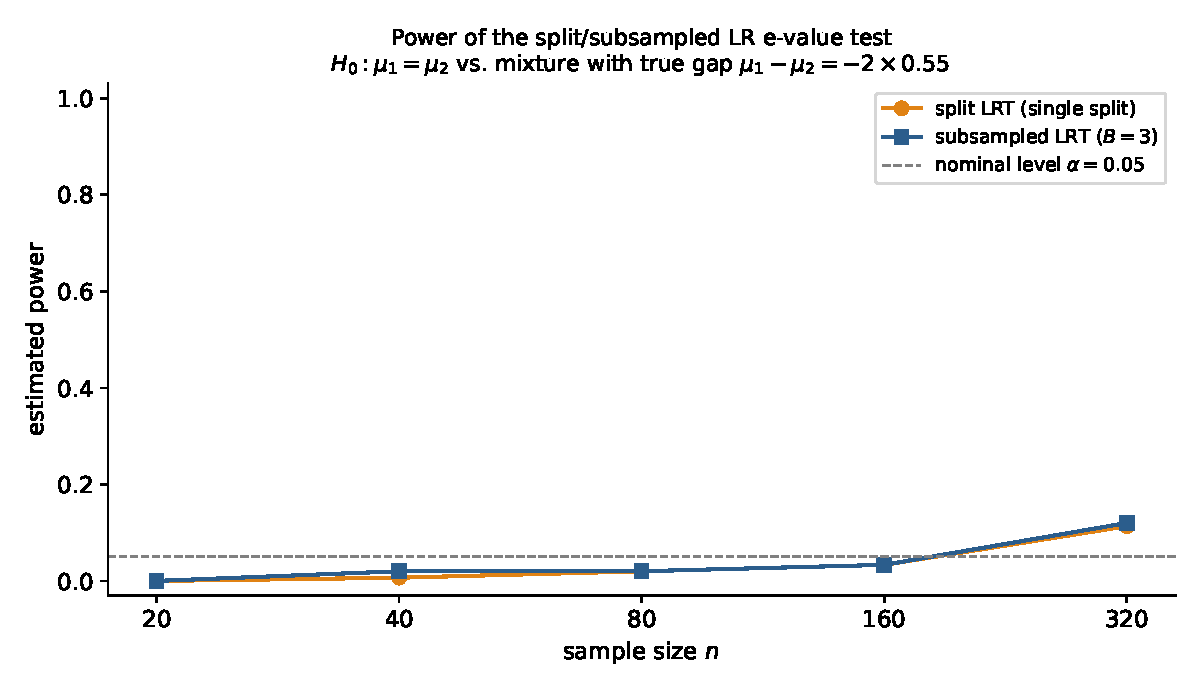
\includegraphics[width=\linewidth]{fig_power_vs_n.pdf}
    \end{column}
    \begin{column}{0.45\textwidth}
      \begin{block}{Results ($150$ reps per $n$)}
        \begin{center}
        \small
        \begin{tabular}{lcc}
          \toprule
          $n$ & split & subsampled ($B{=}3$) \\
          \midrule
          20  & 0.007 & 0.000 \\
          40  & 0.047 & 0.053 \\
          80  & 0.127 & 0.167 \\
          160 & 0.367 & 0.513 \\
          320 & 0.827 & 0.940 \\
          640 & 0.940 & 1.000 \\
          \bottomrule
        \end{tabular}
        \end{center}
      \end{block}
      Exactly as Proposition 5.3/5.4 predict: at every $n$, averaging
      $B=3$ independent splits (subsampled LRT) matches or beats a
      single split, and the gap widens as $n$ grows and power moves
      away from both $0$ and $1$ (where averaging can help the most).
    \end{column}
  \end{columns}

\end{frame}

%==============================================================
\section{Chapter summary}
%==============================================================

\begin{frame}[allowframebreaks]{Chapter 5 summary}

  \begin{block}{The reduction at the heart of the chapter}
    Universal inference reduces composite-vs-composite hypothesis
    testing, under \emph{no regularity conditions}, to computing (or
    upper bounding) the maximum likelihood under the null.
  \end{block}

  \begin{itemize}
    \item \textbf{5.1} Irregular models (unidentified mixture
      parameters, shape constraints like log-concavity) break classical
      asymptotic theory but are exactly where universal inference
      shines.
    \item \textbf{5.2} Split data into $D_0, D_1$; pick $\hat q_1$ on
      $D_1$; fit the null MLE $\hat p_0$ on $D_0$; the ratio
      $E = \prod_{i\in D_0} \hat q_1(X_i)/\hat p_0(X_i)$ is an exact
      e-variable (Theorem 5.1), because $\hat p_0$ dominates $p$
      exactly on the data it is tested against.
    \item \textbf{5.3} Averaging over many independent splits (the
      subsampled/cross-fit e-variable) removes algorithmic randomness
      and can only improve e-power (Jensen/concavity of $\log$), while
      remaining sequentially valid.
    \item \textbf{5.4} The exchangeable Markov inequality (and its
      uniformly-randomized version) is the technical engine that makes
      ``keep splitting until convinced'' a valid, non-cheating stopping
      rule.
    \item \textbf{5.5} Inverting the split LRT point-by-point gives
      universal confidence sets with no regularity conditions, at the
      cost of a small constant-factor inflation versus classical
      (regularity-requiring) sets.
    \item \textbf{5.6} The same idea extends to nuisance parameters,
      unbounded likelihoods (via smoothing), and computationally hard
      MLEs (via relaxations and power likelihoods).
    \item \textbf{5.7} Across every numerical study, the ranking is
      consistent: classical (when available) $>$ subsampling $\approx$
      cross-fit $>$ single split -- but only universal inference remains
      valid when classical asymptotics fail.
  \end{itemize}

\end{frame}

\end{document}
